\noindent
The Latent Cognition Trilogy should be read as the main theoretical sequence within a broader research program on latent cognition, retrieval-native intelligence, and bounded artificial agency. The Trilogy is not an isolated manuscript collection, nor is it a container for every related hypothesis, architectural proposal, or companion paper. Rather, it functions as the central conceptual axis around which a wider body of work is organized.

Within this structure, \textit{Differentiable Latent Indexing in LLMs: Toward Native Retrieval as a Cognitive Function} serves as the architectural foundation of the research program. That work develops the systems-level premise that retrieval should not remain an external augmentation layer, as in conventional retrieval-augmented generation architectures, but may instead be modeled as a differentiable cognitive function embedded within the representational dynamics of transformer-based systems. For this reason, the DLI-LLM paper should be understood as the architectural substrate beneath the Trilogy rather than as a supplementary appendix.

The three companion hypothesis papers occupy a different position. They do not define the program's base architecture. Instead, they formalize adjacent theoretical claims that support, constrain, or extend the main conceptual sequence developed in the Trilogy. Their purpose is to preserve analytical precision around claims that would otherwise overload the central manuscript.

Accordingly, the present work adopts the following canonical structure: the DLI-LLM paper serves as the foundational architecture paper; the Latent Cognition Trilogy constitutes the main theoretical sequence; and the companion hypothesis papers function as formal satellite works within the same research program. This organization allows the Trilogy to remain coherent while preserving the broader intellectual architecture required for future papers, extensions, and domain-specific applications.

\begin{table}[htbp]
\centering
\small
\setlength{\tabcolsep}{4pt}
\renewcommand{\arraystretch}{1.25}
\caption{Canonical organization of the Latent Cognition research program.}
\begin{tabular}{p{0.24\linewidth} p{0.27\linewidth} p{0.38\linewidth}}

\hline
\textbf{Work} & \textbf{Canonical Role} & \textbf{Relationship to the Trilogy} \\
\hline
\textit{Differentiable Latent Indexing in LLMs} & Architectural foundation / formal paper version & Provides the systems-level substrate for Volume I and the broader Trilogy. \\
\hline
Volume I: Memory Fields & Main sequence, first volume & Develops retrieval-native cognition and latent memory fields. \\
\hline
Volume II: Symbolic Stabilization & Main sequence, second volume & Examines how compressed latent representations acquire symbolic stability. \\
\hline
Volume III: Hierarchical Routing & Main sequence, third volume & Analyzes routing as architectural coordination across specialized computation. \\
\hline
Companion Hypothesis Paper I & Formal companion work & Isolates and formalizes a supporting theoretical claim. \\
\hline
Companion Hypothesis Paper II & Formal companion work & Extends the framework into an adjacent conceptual domain. \\
\hline
Companion Hypothesis Paper III & Formal companion work & Tests or constrains the boundaries of the main theoretical sequence.
\\
\hline
Future extensions & Parallel works & Apply or expand the framework into cybersecurity, conscious AI, health sciences, bounded autonomy, or governance-aware AI systems. \\
\hline
\end{tabular}
\end{table}

\begin{figure}[htbp]
    \centering
    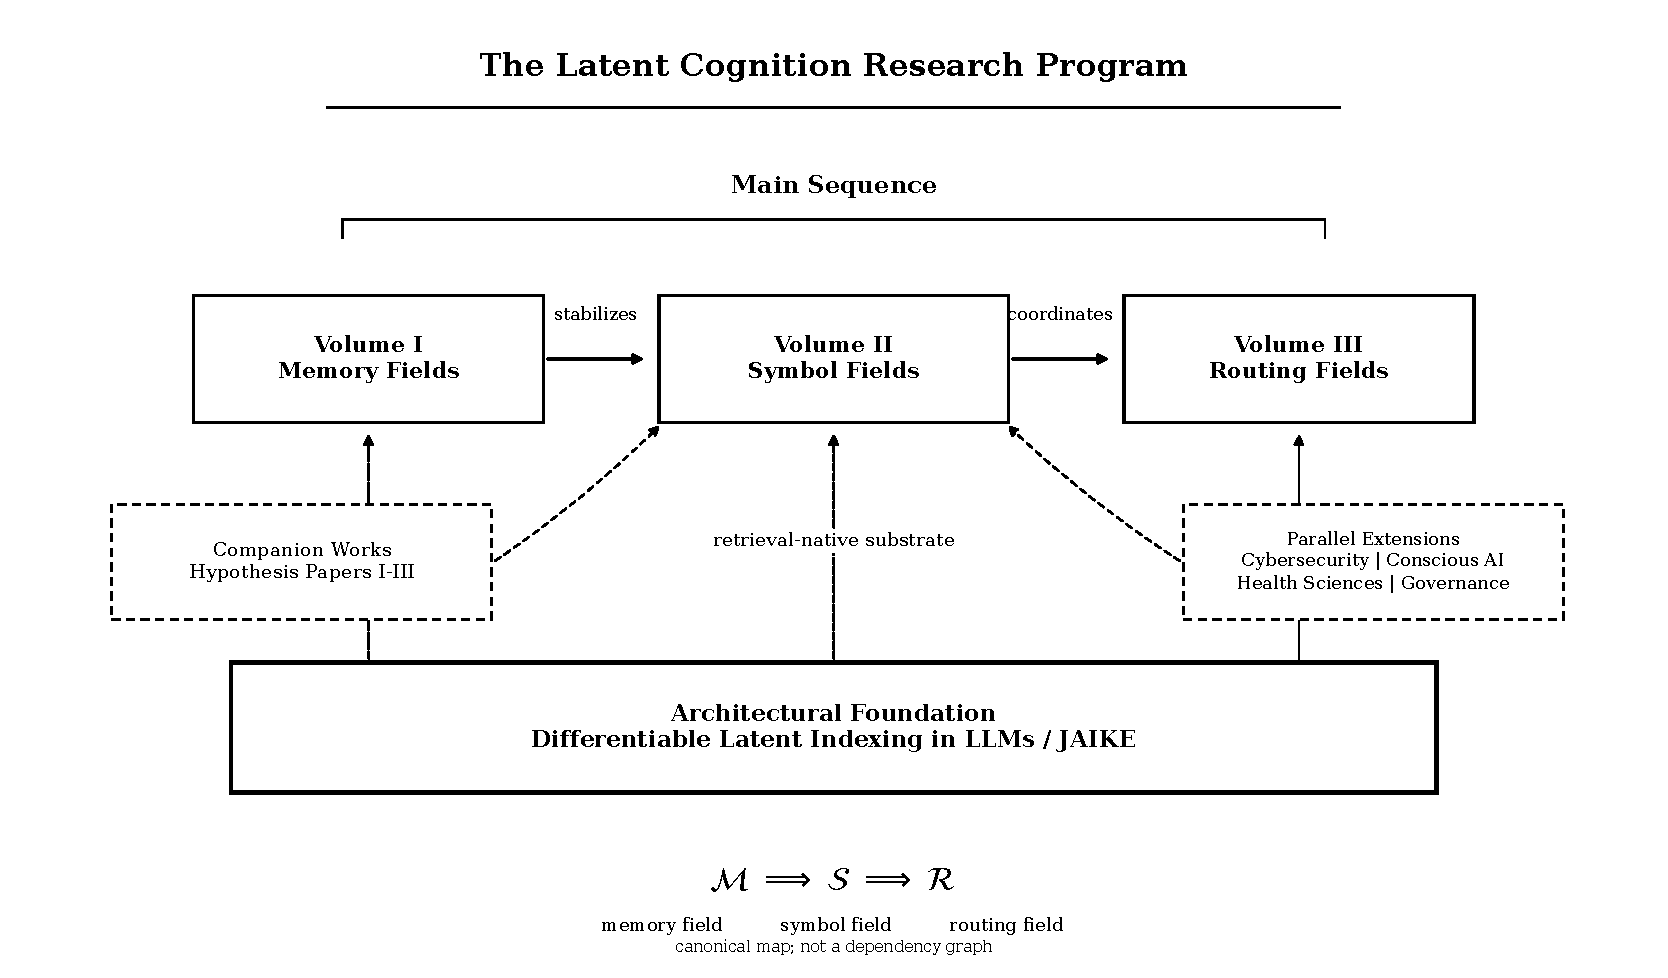
\includegraphics[width=0.88\linewidth]{figures/fig01_trilogy_canonical_map.pdf}
    \caption{Canonical architecture of the Latent Cognition research program. The DLI-LLM manuscript serves as the architectural foundation, while the three volumes of the Trilogy form the main theoretical sequence, progressing from memory fields to symbol fields to routing fields. Companion hypotheses and future extensions orbit the main sequence without replacing it.}
    \label{fig:trilogy-canonical-map}
\end{figure}